\section{Theorie}
\label{sec:Theorie}

Zunächst wird erklärt, wie grundsätzlich Röntgenstrahlung in einer Röntgenröhre entsteht.
Dann werden die grundlegenden Eigenschaften der Brechung an einer Oberfläche erklärt.
Schließlich wird die Reflexion an einer Multischicht erklärt und auch Bezug auf die Rauigkeit und den Geometriefaktor genommen.

\subsection{Entstehung von Röntgenstrahlung} \label{sec:Röntgenstrahlung}

\begin{figure}
    \begin{subfigure}{0.48\textwidth}
        \centering
        \includegraphics[width=\textwidth]{pictures/Aufbau_Rröhre.pdf}
        \caption{Schematische Darstellung einer Röntgenröhre. \cite{demtroeder2}}
        \label{fig:aufbau}
    \end{subfigure}
    \begin{subfigure}{0.48\textwidth}
        \centering
        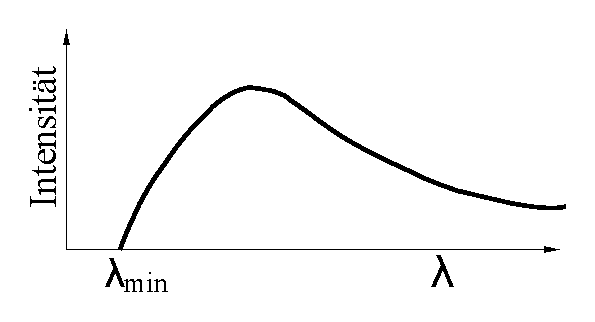
\includegraphics[width=\textwidth]{pictures/bremsspektrum.pdf}
        \caption{Das aufgrund von Energieabgabe kontinuierliche Bremsspektrum des Elektrons. \cite{v602}}
        \label{fig:bremsspektrum}
    \end{subfigure}
    \caption{Aufbau und kontinuierliches Spektrum einer Röntgenröhre.}
\end{figure}

Zur Erzeugung von Röntgenstrahlung werden in einer evakuierten Röhre aus einer Glühkathode
Elektronen emittiert und auf eine Anode hin beschleunigt.
Der schematische Aufbau einer Röntgenröhre ist in \autoref{fig:aufbau} dargestellt.
Die bei der Kollision austretende Strahlung besteht sowohl aus dem kontinuierlichen 
Bremsspektrum, dargestellt in \autoref{fig:bremsspektrum}, 
als auch aus der charakteristischen Röntgenstrahlung des Anodenmaterials.
Bei der Abbremsung eines Elektrons im Coulombfeld des Atomkerns werden Photonen emittiert, 
deren Energie dem Energieverlust den abgebremsten Elektronen entsprechen.
Die minimale Wellenlänge der Photonen bei vollständiger Abbremsung der Elektronen ergibt sich zu
\begin{equation}
    \lambda_\text{min} = \frac{h \cdot c}{e_0 \, U} \,
\end{equation}
wobei die gesamte kinetische Energie $E_\text{kin} = e_0 \, U$ in Strahlungsenergie umgewandelt wird.
Bei der charakteristischen Röntgenstrahlung wird durch Ionisation des Anodenmaterials ein Elektron in ein energetisch höheres Niveau versetzt oder ganz ausgelöst.
Fällt nun ein Elektron von einem energetisch höheren Zustand in ein niedrigeren, wird ein
ein Röntgenquant mit der Energie $h \, \nu = E_\text{m} - E_\text{n}$ emittiert. 
Dies entspricht der Energiedifferenz der beiden Energieniveaus, 
somit besitzt das Röntgenquant eine diskrete Energieverteilung die charakteristisch für das Anodenmaterial der Röntgenröhre.
Diese scharfen Linien werden mit $K_\alpha$, $K_\beta$, $L_\alpha$, ... bezeichnet, wobei $K$, $L$, $M$, ... die Schalen sind, auf denen die Übergänge enden.
Der griechische Buchstabe indexiert die Schale, aus der das Elektron stammt.

\subsection{Grundlagen zur Brechung}
\begin{figure}
    \centering
    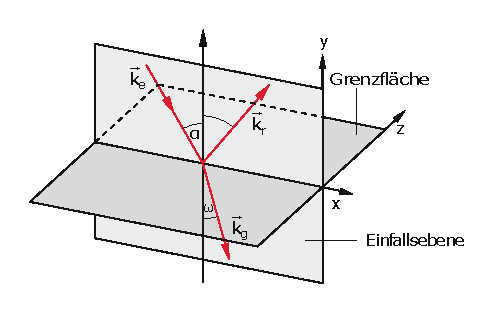
\includegraphics[width=0.6\textwidth]{pictures/Einfall.pdf}
    \caption{Einfall einer elektromagnetischen Welle auf eine Grenzfläche \cite{demtroeder2}.}
    \label{fig:einfall}
\end{figure}
Propagiert eine elektromagnetische Welle in ein anderes Medium, so kommt es zur Brechung.
Dies ist schematisch dargestellt in \autoref{fig:einfall}.
Die Brechung lässt sich durch den Brechungsindex
\begin{equation}
    n = 1 - \delta + i \beta
\end{equation}
beschreiben. Dabei ist $\delta$ ein Korrekturterm und $\beta$ die Absorption des Mediums.
Nun lässt sich mit dem Snelliusschen Brechungsgesetz
\begin{equation}
    \frac{n_1}{n_2} = \frac{\cos (\omega)}{\cos (\alpha)}
\end{equation}
und Vernachlässigung der Absorption die Formel für den kritischen Winkel herleiten, bei dem eine Totalreflexion auftritt.
Dafür setzt man voraus, dass $n_1 = n_\text{Luft} = 1$ ist.
Dann ergibt sich dür kleine $\delta$ \cite{tolan_xray}
\begin{equation}
    \alpha_C \approx \sqrt{2 \delta} = \lambda \sqrt{\frac{r_e \rho}{\pi}} \, .
\end{equation}
Dabei beschreibt $\rho$ die Elektronendichte im Medium und $r_e$ den klassischen Elektronenradius.

Des weiteren lässt sich mithilfe der Fresnelschen Formeln die Transmission und Reflexion von elektromagnetischen Wellen beschreiben.
Dabei lauten die Gleichungen
\begin{align*}
    r_s & =\frac{k_{i,z} - k_{t,z}}{k_{i,z} + k_{t,z}} \, ,\\
    r_p & =\frac{n^2 k_{i,z} - k_{t,z}}{n^2 k_{i,z} + k_{t,z}} \, ,\\
    t_s & =\frac{2 k_{i,z}}{k_{i,z} + k_{t,z}} \, ,\\
    t_p & =\frac{2 k_{i,z}}{n^2 k_{i,z} + k_{t,z}} \, .
\end{align*}
Dabei gilt $k_{i,z} = |k| \sin \alpha_i$ und $k_{t,z} = n |k| \sin \alpha_t$.
Da bei Röntgenstrahlung $n \approx 1$ ist, gilt $r_s = r_p$ und $t_s = t_p$.
Hieraus lässt sich dann der Fresnelsche Reflexionskoeffizient bestimmen.
Dieser ist bei $\alpha_i > 3 \alpha_C$ näherungsweise gegeben als \cite{tolan_xray}
\begin{equation}
    R\approx \left( \frac{\alpha_C}{2 \alpha_i} \right)^4 \, .
\end{equation}

\subsection{Reflektivität an Multischichtsystemen}

\begin{figure}
    \begin{subfigure}{0.38\textwidth}
        \centering
        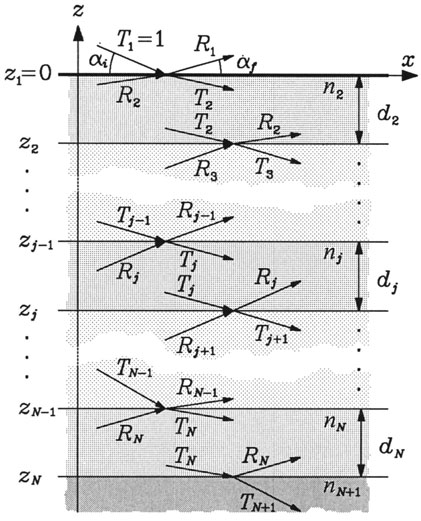
\includegraphics[width=\textwidth]{pictures/multischicht.pdf}
        \caption{Darstellung einer Mehrfachreflexion an einer Multischicht \cite{tolan_xray}.}
        \label{fig:multischicht}
    \end{subfigure}
    \begin{subfigure}{0.58\textwidth}
        \centering
        \includegraphics[width=\textwidth]{pictures/kiessig.pdf}
        \caption{Schematische Darstellung von Kiessig-Osz. . \cite{kiessig}}
        \label{fig:kiessig}
    \end{subfigure}
    \caption{Abbildungen zu einer Multischichtreflexion.
    \label{fig:subkiessig}}
\end{figure}

Liegt ein Multischichtsystem vor, so kommt es zu den sogenannten \enquote{Kiessig-Oszillationen}.
Die Kiessig-Oszillationen sind in \autoref{fig:kiessig} abgebildet.
Die Kiessig-Oszillationen entstehen aufgrund von Interferenzeffekten an der Oberfläche.
Diese Interferenzen entstehen durch die Überlagerung der Reflexion an verschiedenen Schichten.
Bei einer destruktiven Interferenz liegt ein Phasenunterschied von $\frac{\lambda}{2}$ oder einem ungeraden vielfachen davon vor.
Aus der Gleichung
\begin{equation} \label{eq:schichtdicke}
    d = \frac{\lambda}{2 \Delta \alpha_i}
\end{equation}
lässt sich dann der Abstand der Ebenen bestimmen.
Dabei beschreibt $\Delta \alpha_i$ die Periodenlänge einer Oszillation. 
Lässt sich das System durch N+1 Schichten wie in \autoref{fig:multischicht} beschreiben, lässt sich der Parratt-Algorithmus anwenden \cite{tolan_xray}.
Dabei handelt es sich um einen rekursiven Ansatz, der bei der Berechnung der untersten Schicht beginnt.
Der Ansatz ist dabei, dass bei einer \enquote{unendlich tiefen} Schicht die Strahlung nicht mehr reflektiert wird.
Die Rekursionsformel lautet
\begin{equation}
    X_j=\frac{R_j}{T_j}=\exp \left(-2 \mathrm{i} k_{z, j} z_j\right) \frac{r_{j, j+1}+X_{j+1} \exp \left(2 \mathrm{i} k_{z, j+1} z_j\right)}{1+r_{j, j+1} X_{j+1} \exp \left(2 \mathrm{i} k_{z, j+1} z_j\right)} \, .
\end{equation}
In der Formel bezeichnet $r_{j,j+1}$ die Fresnelreflektivität an der $j$-ten Grenzfläche.

Als nötige Modifikation des Parratt-Algorithmus gilt die Rauigkeit.
Denn im Algorithmus wurde angenommen, dass die Oberflächen perfekt glatt sind.
Dies ist bei realen Objekten nicht der Fall.
Diese Rauigkeit kann durch eine Anpassung der Fresnelkoeffizienten ausgeglichen werden.
Diese lauten
\begin{align}
    & \tilde{r}_{j, j+1}=r_{j, j+1} \exp \left(-2 k_{z, j}^2 \sigma_j^2\right) \, ,\\
    & \tilde{t}_{j, j+1}=t_{j, j+1} \exp \left\{-\left(k_{z, j}-k_{z, j+1}\right)^2 \sigma_j^2 / 2\right\} \, .
\end{align}
Das $\sigma_j^2$ beschreibt die sogenannte \enquote{root-mean-squre roughness}.
Diese wiederum ist definiert als
\begin{equation*}
    \sigma_j^2 = \int (z - \mu_j)^2 P_j (z) dz \, .
\end{equation*}

\subsection{Der Geometriefaktor/- und Winkel}
\begin{figure}
    \centering
    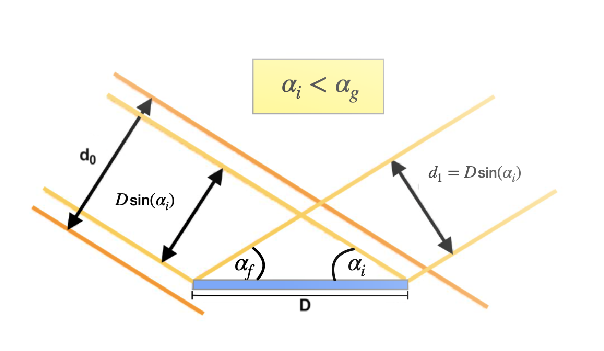
\includegraphics[width=0.6\textwidth]{pictures/geometriefaktor.pdf}
    \caption{Geometrie des Strahlenverlaufs \cite{v44}.}
    \label{fig:geometriefaktor}
\end{figure}
Fällt der Strahl auf die Probe, so ist er größer als die Probe selbst.
Dies ist in \autoref{fig:geometriefaktor} zu erkennen.
Durch einführen des Geometriefaktors $G$ kann die Differenz der Strahlungsintensität nach der Reflexion berücksichtigt werden. 
Er lautet
\begin{equation} \label{eq:geometriefaktor}
    G= \begin{cases}\frac{D \sin \alpha_{\mathrm{i}}}{d_0} & \text { für } \alpha_{\mathrm{i}}<\alpha_{\mathrm{g}} \\ 1 & \text { für } \alpha_{\mathrm{i}} \geq \alpha_{\mathrm{g}}\end{cases} \, .
\end{equation}
Dabei ist $D$ der Durchmesser der Probenoberfläche, $d_0$ die Höhe des Strahls, $\alpha_i$ der Einfallswinkel und $\alpha_G$ ist der Winkel, unter dem keine Intensität mehr
durch geometrische Eigenschaften verloren geht.